\documentclass[11pt]{report}
\usepackage[utf8]{inputenc}
\usepackage[T1]{fontenc}
\usepackage[italian]{babel}
\usepackage{graphicx}
\graphicspath{ {./img/} }
\usepackage{tabularx}
\usepackage{titlesec}
\usepackage{multicol}
\usepackage{tikz}
\usepackage{geometry}
\geometry{
	a4paper, 
	left=20mm,
	right=20mm,
	top=20mm,
	bottom=20mm
}
\usepackage{hyperref}


% Template
\usepackage{noteTemplate}
\usepackage{titlepage}

\begin{document}
\customtitlepage
\newpage
\tableofcontents

\chapter{PostgreSQL}

\section{Introduzione}

PostgreSQL è un RDBMS con alcune funzionalità orientate agli oggetti. E' multipiattaforma, opensource e gestito da un gruppo di volontari. La documentazione si pu\`o trovare sul sito ufficiale di \url{http://www.postgresql.org}.
PostgreSQL implementa gran parte dello standard SQL: la versione 16 implementa quasi tutte le funzioni SQL 2023, per approfondire si rimanda alla \href{https://www.postgresql.org/docs/16/features.html}{documentazione}.

L'interazione tra un utente e le basi di dati gestite da PostgreSQL avviene secondo il modello \emph{client-server}.

\subsection{Server} 
Il daemon postmaster supervisiona tutti i processi specifici di PostgreSQL.
\subsection{Client(s)} 
Qualsiasi programma in grado di gestire l'interazione con postmaster (input di comandi, invio al postmaster, visualizzazione esito comando, ecc).
Il client standard \`e \textbf{psql}, un'applicazione a linea di comando. Esiste un'alternativa interessante: \href{http://www.pgadmin.org}{\textbf{pgAdmin IV}}, un client grafico pi\`u intuitivo.

\subsection{Esempio di connessione al server tramite psql}
\begin{lstlisting}
psql -h db-srv.di.univr.it -U <userid> <nomeid>
Inserisci la password per l`utente <userid>
psql(16.0)
connessione SSL (protocollo: TLSv1.2, cifrario ECDHE-RSA-AES256-GCM-SHA384, 
bit: 256, compressione: disattivato)

Digita 'help' per avere un aiuto
<usrid> =>
\end{lstlisting}

\textbf{psql} \`e un interprete iterativo da terminale. Accetta due tipi di comando: comando di tipo SQL (Structured Query Language) o comandi interni.
\begin{itemize}
\item Comandi SQL: permettono di creare/gestire e interrogare le basi di dati.
\item Comandi interni (riconoscibili perch\'e iniziano con '\\'): permettono di configurare il client o avere aiuto per scrivere comandi SQL.
\end{itemize}

\section{Esempio applicativo psql}
\begin{center}
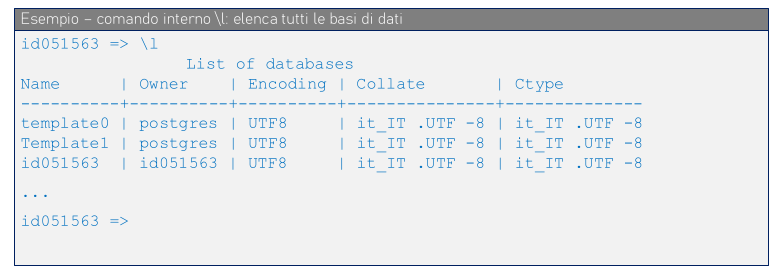
\includegraphics[scale=0.5]{applicativo-psql.png}

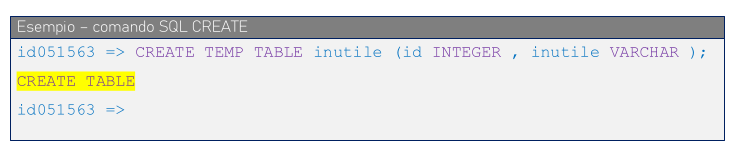
\includegraphics[scale=0.525]{applicativo-psql-esempio-sql.png}
\end{center}


\chapter{Structured Query Language - SQL}
\section{Notazione}
\begin{itemize}
\item \textbf{[} e \textbf{]} indicano parti opzionali, il termine pu\`o non comparire o comparire una sola volta;
\item \textbf{\{} e \textbf{\}} indicano che il termine pu\`o non comparire o comparire un numero arbitrario di volte;
\item L'istruzione \texttt{CREATE TABLE} definisce uno schema di relazione e ne crea un'istanza vuota: attributi, domini e vincoli.

\end{itemize}

\section{Creazione di una tabella}
Esempio di sintassi per la creazione di una tabella:
\begin{lstlisting}{language=SQL}
CREATE TABLE tabella {
	attributo dominio [ valoreDefault ] { vincolo }
	{, attributo dominio [valoreDefault } { vincolo } }
	{, vincoloTabella }
]);
\end{lstlisting}

\section{Domini elementari}

\subsection{Caratteri}

Permette di rappresentare singoli caratteri oppure stringhe. Un carattere o una stringa di caratteri sono rappresentati tra apici singoli, ad esempio \texttt{'a'} oppure \texttt{'questa \`e una stringa'}.

La lunghezza delle stringhe pu\`o essere fissa o variabile.

\begin{lstlisting}{language=SQL}
CHARACTER [VARYING] [(lunghezza)]

CHARACTER				-- carattere singolo
CHARACTER(20)			-- stringa di lunghezza fissa, se si inseriscono meno di 20 caratteri viene riempita di spazi.
CHARACTER VARYING(20) 	-- stringa di lunghezza variabile, max 20 caratteri.
TEXT					-- stringa di lunghezza variabile senza limite fissato. Estensione PostgreSQL
\end{lstlisting}

\subsection{Boolean}

Permette di rappresentare i valori booleani \texttt{TRUE/FALSE}, rappresentati anche come \texttt{t/f, 1/0, yes/NO}, pi\`u lo stato unkonown (valore nullo), rappresentato come \texttt{NULL}.

\begin{lstlisting}{language=SQL}
BOOLEAN 		-- valore booleano singolo
\end{lstlisting}

\subsection{Tipi numerici esatti}

Permettono di rappresentare valori esatti interi o con parte decimale di lunghezza prefissata.

\subsubsection{Valori interi}

\begin{lstlisting}{language=SQL}
SMALLINT 		-- valori interi (2 bytes da -32768 a +32767)
INTEGER 		-- valori interi (4 bytes da - 2147483648 a +2147483647)
\end{lstlisting}

\subsubsection{Valori decimali}

\begin{lstlisting}{language=SQL}
NUMERIC [ (precisione [, scala]) ]
\end{lstlisting}

Dove \textbf{precisione} \`e il numero totale di cifre significative, cio\`e sia a sinistra che a destra della virgola; mentre \textbf{scala} \`e il numero di cifre dopo la virgola, se vuoto = 0.
Equivalente a \texttt{NUMERIC} esiste anche il tipo \texttt{DECIMAL}:
\begin{lstlisting}{language=SQL}
DECIMAL [ (precisione [, scala]) ]
\end{lstlisting}

\paragraph{Esempio} utilizzo di \texttt{NUMERIC}:
\begin{lstlisting}{language=SQL}
NUMERIC(5,2) -- permette di rappresentare valori come 100.01 o 100.99 (arrotondato a 101.00) 
-- ma non rappresenta valori come 1000.01
\end{lstlisting}

\subsection{Tipi numerici approssimati}

Permettono di rappresentare valori in virgola mobile. \

\begin{lstlisting}{language=SQL}
REAL -- precisione di 6 cifre decimali.

DOUBLE PRECISION -- precisione di 15 cifre decimali.
\end{lstlisting}

Ciascun numero \`e rappresentato da una coppia di valori: la mantissa e l'esponente. La mantissa \`e un numero frazionario, l'esponente \`e un numero intero. Il valore si ottiene moltiplicando la mantissa per la potenza di 10 con grado pari all'esponente, ad esempio:
$ 0.176E16 = 1.7 \times 10^{15}$ oppure $-0,4E-6 = -4 \times 10^{-7}$

\textbf{Nota}: \texttt{REAL} e \texttt{DOUBLE PRECISION} sono comunque valori approssimati. Se si devono rappresentare importi di denaro che contengono anche decimali, \textbf{mai usare questi tipi, ma usare \texttt{NUMERIC(precisione)}}.

\subsection{Istanti temporali}

Permettono di rappresentare gli istanti di tempo

\subsubsection{DATE}
Un valore \texttt{DATE} si rappresenta tra apici (') e lo standard ISO prescrive il formato YYYY-MM-DD.
\begin{lstlisting}{language=SQL}
DATE 								-- anno, mese, giorno
\end{lstlisting}

\subsubsection{TIME}
Istanti del tipo hour, minute, second. Precisione \`e il numero di cifre decimali per rappresentare frazioni del secondo.
\texttt{WITH TIME ZONE} permette di specificare anche $\pm$hour, minute, che rappresentano la differenza con l'ora di Greenwich, o nomeFusoOrario.
\begin{lstlisting}{language=SQL}
TIME [ (precisione)] [WITH TIME ZONE]	-- hour, minute, second
\end{lstlisting}

\subsubsection{TIMESTAMP}
\begin{lstlisting}{language=SQL}
TIMESTAMP [ (precisione)] [WITH TIME ZONE]	-- date + time
\end{lstlisting}

\subsection{Intervalli temporali}
Permettono di rappresentare intervalli di tempo, come la durata di un evento. La sintassi \`e
\begin{lstlisting}{language=SQL}
INTERVAL primaUnitaDiTempo [TO ultimaUnitaDiTempo]
\end{lstlisting}
\texttt{primaUnitaDiTempo} e \texttt{ultimaUnitaDiTempo} definiscono le unit\`a di misura che deveono essere utilizzate, dalla pi\'u precisa alla meno precisa. Esempio:
\begin{lstlisting}{language=SQL}
INTERVAL year TO month -- indica un intervallo di tempo misurato in numero di anni e mesi
\end{lstlisting}

L'insieme delle unit\`a di misura \`e diviso in due insiemi distinti: da \emph{year} a \emph{month} e da \emph{day} a \emph{second}.
Poich\'e non \`e possibile paragonare esattamente giorni e mesi (un mese pu\`o avere da 28 a 31 giorni).

Si pu\`o specificare una precisazione per la \texttt{primaUnitaDiTempo}: numero di cifre in base 10 per la \textbf{rappresentazione}.
Se l'\texttt{ultimaUnitaDiTempo} \`e \textbf{second}, si pu\`o specificare una precisione che rappresenta il numero di cifre decimali dopo la virgola. Ad esempio:
\begin{lstlisting}{language=SQL}
INTERVAL year(5) TO month -- intervalli della durata fino a 99 999 anni e 11 mesi

INTERVAL day(4) TO second(2) -- intervalli della durata fino a 9999 giorni, 23 ore, 59 minuti e 59.99 secondi
\end{lstlisting}

\section{Domini definiti dall'utente}

L'istruzione \texttt{CREATE DOMAIN} definisce un dominio, utilizzabile in definizioni di relazioni, anche con vincoli e valori di default. Il dominio pu\`o essere definito a partire da un dominio elementare oppure da un altro dominio definito dall'utente. 

\textbf{Sintassi:}
\begin{lstlisting}{language=SQL}
CREATE DOMAIN nome AS tipoBase [valoreDefault] [vincolo]
\end{lstlisting}

Per esempio creiamo il dominio \texttt{giorniSettimana} che indica i giorni della settimana con 3 caratteri:
\begin{lstlisting}{language=SQL}
CREATE DOMAIN giorniSettimana AS CHARACTER(3)
	CHECK (VALUE IN ('LUN', 'MAR', 'MER', 'GIO', 'VEN', 'SAB', 'DOM'));
\end{lstlisting}

Un altro esempio potrebbe essere un dominio per rappresentare un voto:
\begin{lstlisting}{language=SQL}
CREATE DOMAIN Voto
	AS SMALLINT
	DEFAULT NULL
	CHECK ( value >= 18 AND value <=30);
\end{lstlisting}

\section{Vincoli intrarelazionali}

Abbiamo quattro vincoli intrarelazionali: 
\begin{itemize}
\item \texttt{NOT NULL}: il valore nullo non \`e ammesso per l'attributo, quindi il valore deve sempre essere specificato, o si assegna un valore di default.
\item \texttt{UNIQUE}: definisce (super)chiavi.
\item \texttt{PRIMARY KEY}: chiave primaria (una sola, implica \texttt{NOT NULL}).
\item \texttt{CHECK}
\end{itemize}

\subsection{Vincolo \texttt{NOT NULL} e \texttt{DEFAULT}}

Il vincolo \texttt{NOT NULL} determina che il valore nullo non \`e ammesso come valore dell'attributo. Nel caso di vincoli \texttt{NOT NULL} pu\`o essere utile specificare un valore di default per l'attributo. 

L'istruzione \texttt{DEFAULT valore} specifica un valore di default per un attributo quando un comando di inserimento dati non specifica nessun valore per l'attributo.
\newline

\noindent\textbf{Esempio:}

\begin{lstlisting}{language=SQL}
nome VARCHAR(20) NOT NULL
cognome VARCHAR(20) NOT NULL DEFAULT 'VUOTO'
\end{lstlisting}

\subsection{Vincolo \texttt{UNIQUE}}

Il vincolo \texttt{UNIQUE} impone che righe differenti della tabella non possono avere gli stessi valori: concetto di superchiave il quale, per\`o, richiede anche il vincolo di \texttt{NOT NULL}.

Si pu\`o definire su un solo attributo o su un insieme di attributi. 

\begin{center}
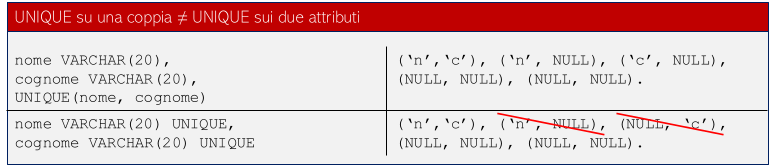
\includegraphics[scale=0.5]{vincolo-unique}
\end{center}

\subsection{Vincolo \texttt{PRIMARY KEY}}

Il vincolo \texttt{PRIMARY KEY} identifica l'attributo che rappresenta la chiave primaria della relazione. Si usa una volta per tabella ed implica il vincolo \texttt{NOT NULL}.

Esistono due forme per la specifica:
\begin{itemize}
\item nella definizione dell'attributo, se \`e l'unico componente della chiave primaria;
\begin{lstlisting}{language=SQL}
matricola CHAR(6) PRIMARY KEY;
\end{lstlisting}
\item come definizione separata a livello di tabella (vincolo di tabella), se invece la \emph{chiave primaria} \`e composta da pi\`u attributi.
\begin{lstlisting}{language=SQL}
nome VARCHAR(20),
cognome VARCHAR(20), 
PRIMARY KEY(nome, cognome);
\end{lstlisting}
\end{itemize}
\newpage
\subsection{Vincolo \texttt{CHECK}}

Il vincolo \texttt{CHECK} specifica un vincolo generico che devono soddisfare le tuple della tabella. Un vincolo \texttt{CHECK} è soddisfatto se la sua espressione è vera o nulla.

\begin{lstlisting}{language=SQL}
CREATE TABLE Impiegato (
matricola CHAR(6) PRIMARY KEY,
nome VARCHAR(20) NOT NULL,
cognome VARCHAR(20) NOT NULL,
qualifica VARCHAR(20),
stipendio NUMERIC(8,2) DEFAULT 500.00 NOT NULL
CHECK( stipendio >= 0.0 ), --check di attributo
UNIQUE( cognome, nome ),
CHECK( nome <> cognome ) --check di tabella
);
\end{lstlisting}

\section{Vincoli interrelazionali}

Un vincolo di \textbf{integrità referenziale} (o interrelazionale) crea un legame tra i valori di un attributo, o di un insieme di essi, $A$ della tabella corrente (detta interna/slave) e i valori di un attributo, o di un insieme di essi, $B$ di un'altra tabella (detta esterna/master).

Il vincolo interrelazionale impone che, in ogni tupla della tabella interna, il valore di $A$, \textbf{se diverso dal valore nullo}, sia presente tra i valori di $B$ nella tabella esterna.
L'attributo $B$ della tabella esterna deve essere soggetto a un vincolo \texttt{UNIQUE} o \texttt{PRIMARY KEY}. 

\examplebox{\paragraph{Nota:} l'attributo (o insieme di attributi) $B$ pu\`o anche non essere la chiave primaria, ma deve essere identificante per le tuple della tabella esterna.}

Le keyword \texttt{REFERENCES} e \texttt{FOREIGN KEY} permettono di definire vincoli di integrit\`a referenziale. 

\subsection{Sintassi per singoli attributi}

Se \`e coinvolto un singolo attributo, basta usare il costrutto sintattico \texttt{REFERENCES} nella dichiarazione dell'attributo, specificando la tabella esterna e il relativo attributo coinvolto.

\begin{lstlisting}{language=SQL}
CREATE TABLE Impiegato (
	Matricola = CHARACTER(6) PRIMARY KEY, 
	Nome = CHARACTER VARYING(20) NOT NULL, 
	Cognome = CHARACTER VARYING(20) NOT NULL, 
	Dipart = CHARACTER VARYING(15) 
				REFERENCES Dipartimento(NomeDip), -- singolo attributo
	Ufficio = NUMERIC(3),
	Stipendio = NUMERIC(9) DEFAULT 0, 
	UNIQUE (Cognome, Nome)
);
\end{lstlisting}

\subsection{Sintassi per pi\`u attributi}

Quando il legame coinvolge pi\`u attributi si usa il costrutto \texttt{FOREIGN KEY} alla fine della definizione degli attributi, elencando gli attributi coinvolti e seguito dalla definizioni dei corrispondenti attributi della tabella esterna, sempre grazie a \texttt{REFERENCES}.
\newpage
\begin{lstlisting}{language=SQL}
CREATE TABLE Impiegato (
	Matricola = CHARACTER(6) PRIMARY KEY, 
	Nome = CHARACTER VARYING(20) NOT NULL, 
	Cognome = CHARACTER VARYING(20) NOT NULL, 
	Dipart = CHARACTER VARYING(15) 
				REFERENCES Dipartimento(NomeDip),
	Ufficio = NUMERIC(3),
	Stipendio = NUMERIC(9) DEFAULT 0, 
	FOREIGN KEY(Nome, Cognome) REFERENCES Anagrafica (Nome, Cognome) -- due attributi
);
\end{lstlisting}

\section{Esempio di creazione di una tabella}

\begin{center}
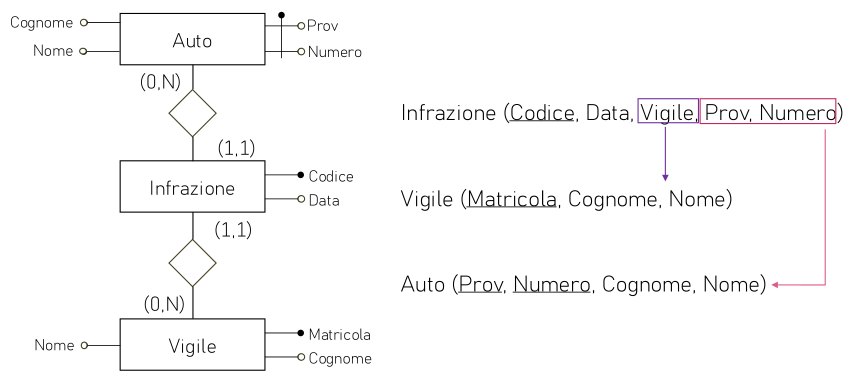
\includegraphics[scale=0.5]{example-create}
\end{center}

\begin{lstlisting}{languate=SQL}
CREATE TABLE Infrazione (
	Codice CHAR(6) PRIMARY KEY,
	Data DATE NOT NULL, 
	Vigile INTEGER NOT NULL
			REFERENCES Vigile(Matricola), 
	Provincia CHAR(2), 
	Numero CHAR(6), 
	FOREIGN KEY(Provincia, Numero)
			REFERENCES Auto(Provincia, Numero)
);
\end{lstlisting}

\section{Modifiche degli schemi}

L'SQL offre delle primitive per modificare schemi gi\`a introdotti. Il comando \texttt{ALTER} effettua modifiche a domini e tabelle. Ad esempio, \`e possibile aggiungere una colonna a una relazione.
Il comando \texttt{DROP (DOMAIN/TABLE)} permette di rimuovere i vari componenti di domini e tabelle. Ad esempio \`e possibile cancellare una tabella.

\subsection{Comando \texttt{ALTER TABLE}}

La struttura di una tabella si pu\`o modificare dopo la sua creazione con questo comando. Le modifiche pi\`u comuni sono: 

\begin{itemize}
\item Aggiunta di un nuovo attributo \texttt{ADD COLUMN}
\begin{lstlisting}{language=SQL}
-- Sintassi
ALTER TABLE tabella ADD COLUMN attributo tipo;
-- Esempio
ALTER TABLE impiegato ADD COLUMN stipendio NUMERIC(8,2);
\end{lstlisting}
\item Rimozione di un attributo \texttt{DROP COLUMN}
\begin{lstlisting}{language=SQL}
-- Sintassi
ALTER TABLE tabella DROP COLUMN attributo;
\end{lstlisting}
\item Modifica valore di default di un attributo \texttt{ALTER COLUMN}
\begin{lstlisting}{language=SQL}
-- Sintassi
ALTER TABLE tabella ALTER COLUMN attributo { SET DEFAULT valore | DROP DEFAULT};
-- Esempio
ALTER TABLE impiegato ALTER COLUMN stipendio SET DEFAULT 1000.00;
\end{lstlisting}
\end{itemize}

\section{Cancellazione dati in una tabella}

Le tuple di una tabella vengono cancellate con il comando \texttt{DELETE}:
\begin{lstlisting}{language=SQL}
DELETE FROM tabella [WHERE condizione ];
\end{lstlisting}

La \textbf{condizione} \`e un'espressione booleana che seleziona quali tuple cancellare. Se \texttt{WHERE} non \`e presente, tutte le tuple saranno cancellate, infatti una tabella viene cancellata con il comando \texttt{DROP TABLE}:
\begin{lstlisting}{language=SQL}
DROP TABLE tabella;
\end{lstlisting}

\subsubsection{Esempi}

\begin{lstlisting}{language=SQL}
-- Cancellazione di una tupla
DELETE FROM impiegato 	WHERE matricola = 'A001';

-- Cancellazione di una tabella
DROP TABLE impiegato;
\end{lstlisting}




































\end{document}